\documentclass[12pt]{article}

% a template that a friend gave, it's worked well enough for me
% i have added some packages and stuff that have proved useful

\usepackage{fancyhdr}
\usepackage{tipa}
\usepackage{fontspec}
\usepackage{amsfonts}
\usepackage{enumitem}
\usepackage[margin=1in]{geometry}
\usepackage{graphicx}
\usepackage{float}
\usepackage{amsmath}
\usepackage{braket}
\usepackage{amssymb}
\usepackage{booktabs}
\usepackage{hyperref}
\usepackage{mathtools}
\usepackage{xcolor}
\usepackage{float}
\usepackage{algpseudocodex}
\usepackage{titlesec}
\usepackage{bbm}

\pagestyle{fancy}
\fancyhf{} % sets both header and footer to nothing
\lhead{Kevin Sheng}
\setmainfont{Comic Neue}
\renewcommand{\headrulewidth}{1pt}
\setlength{\headheight}{0.75in}
\setlength{\oddsidemargin}{0in}
\setlength{\evensidemargin}{0in}
\setlength{\voffset}{-.5in}
\setlength{\headsep}{10pt}
\setlength{\textwidth}{6.5in}
\setlength{\headwidth}{6.5in}
\setlength{\textheight}{8in}
\renewcommand{\headrulewidth}{0.5pt}
\renewcommand{\footrulewidth}{0.3pt}
\setlength{\textwidth}{6.5in}
\usepackage{setspace}
\usepackage{multicol}
\usepackage{float}
\setlength{\columnsep}{1cm}
\setlength\parindent{24pt}
\usepackage [english]{babel}
\usepackage [autostyle, english = american]{csquotes}
\MakeOuterQuote{"}

\setlength{\parskip}{6pt}
\setlength{\parindent}{0pt}

\titlespacing\section{0pt}{12pt plus 4pt minus 2pt}{0pt plus 2pt minus 2pt}
\titlespacing\subsection{0pt}{12pt plus 4pt minus 2pt}{0pt plus 2pt minus 2pt}
\titlespacing\subsubsection{0pt}{12pt plus 4pt minus 2pt}{0pt plus 2pt minus 2pt}

\hypersetup{colorlinks=true, urlcolor=blue}

\newcommand{\correction}[1]{\textcolor{red}{#1}}


\rhead{ECE 102}

\begin{document}

\begin{enumerate}
      \item \begin{enumerate}
                  \item \begin{enumerate}
                              \item 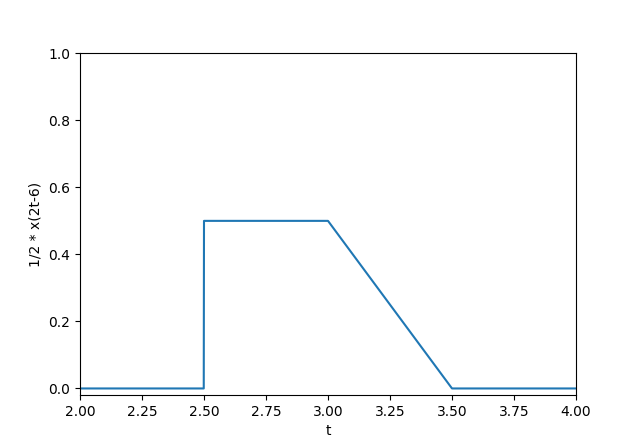
\includegraphics[width=12cm]{img/hw1/i}
                              \item 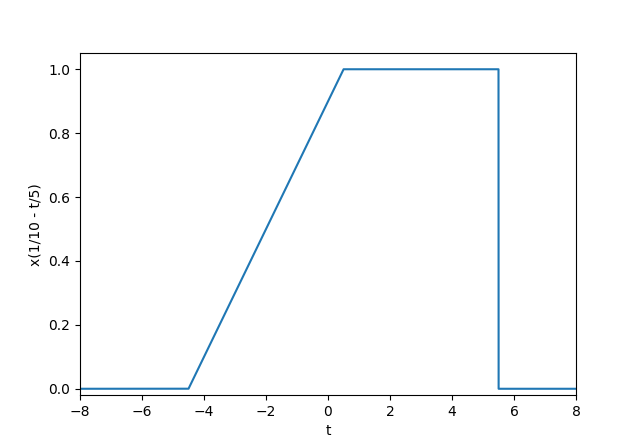
\includegraphics[width=12cm]{img/hw1/ii}
                        \end{enumerate}
                  \item This graph corresponds to a shift to the right by $\frac{3}{2}$
                        followed by a scale of $-\frac{1}{2}$.
                        Thus, this graph is of the signal $\boxed{x\left(-\frac{1}{2}t-\frac{3}{2}\right)}$.
            \end{enumerate}
      \item \begin{enumerate}
                  \item Suppose $f$ and $g$ are two odd functions.
                        Let $h$ be their product. Then,
                        \begin{align*}
                              h(x) & = f(x) \cdot g(x)     \\
                                   & = -f(-x) \cdot -g(-x) \\
                                   & = f(-x) \cdot g(-x)   \\
                                   & = h(-x)\quad\square
                        \end{align*}
                  \item Let the setup be the same as in the previous question, except now $f$ is even.
                        \begin{align*}
                              h(x) & = f(x) \cdot g(x)    \\
                                   & = f(-x) \cdot -g(-x) \\
                                   & = -f(-x) \cdot g(-x) \\
                                   & = -h(-x)\quad\square
                        \end{align*}
                  \item Apply the formula taught in lecture. (lmao)
                        \begin{align*}
                              x_e(t) & = \frac{x(t)+x(-t)}{2}                                                                                                                  \\
                                     & = \frac{1}{2} \left[t \sin t + t^3 \left(\frac{e^t+e^{-t}}{2}\right)+2024-t \sin (-t)-t^3 \left(\frac{e^{-t}+e^t}{2}\right)+2024\right] \\
                                     & = \boxed{t \sin t + 2024}                                                                                                               \\
                              \\
                              x_o(t) & = x(t) - x_e(t)                                                                                                                         \\
                                     & =\boxed{t^3 \left(\frac{e^t+e^{-t}}{2}\right)}
                        \end{align*}
            \end{enumerate}
      \item \begin{enumerate}
                  \item \begin{enumerate}
                              \item Periodic with $f=30$.
                              \item Using that $\cos^2(x)=\frac{\cos(2x)+1}{2}$, we can change this expression to
                                    \[x(t)=10\cos^2\left(\frac{\pi}{2}t\right)=5(\cos(\pi t)+1)\]
                                    From this, we can see that the signal is periodic with $f=\boxed{\frac{1}{2}}$.
                              \item Not periodic, since $\frac{2/5}{1/8\pi}$ is irrational.
                              \item Not periodic, since the right and left halves are fundamentally different and never mirror each other perfectly.
                        \end{enumerate}
                  \item Since $x$ is odd, $x(0)=-x(0)=0$.
                        Also, since $x(T_0)=x(T_0-nT_0)$ where $n$ is any integer, $x(T_0)=x(0)=\boxed{0}$.
                  \item The signal remains unchanged.
                  \item Yes, it is periodic with $T_0'=\frac{T_0}{5}$.
                        This is because
                        \begin{align*}
                              x\left(5\left(t+\frac{T_0}{5}\right)+2\right)
                               & = x(5t+T_0+2)         \\
                               & = x((5t+2)+T_0)       \\
                               & = x(5t+2)\quad\square
                        \end{align*}
            \end{enumerate}
      \item \begin{enumerate}
                  \item \begin{enumerate}
                              \item Before we begin, note that $\left(e^{-|t|}\right)^2=e^{-2|t|}$
                                    \begin{align*}
                                          \int_{-\infty}^{\infty} e^{-2|t|}\,dt
                                           & = \int_{-\infty}^{0} e^{2t}\,dt + \int_{0}^{\infty} e^{-2t}\,dt                                                          \\
                                           & = \left.\left(\frac{1}{2}e^{2t}\right)\right|^{0}_{-\infty} + \left.\left(-\frac{1}{2}e^{-2t}\right)\right|^{\infty}_{0} \\
                                           & = \frac{1}{2}+\frac{1}{2}                                                                                                \\
                                           & = \boxed{1}
                                    \end{align*}
                                    This is an energy signal.
                              \item $x(t)^2$ is $\frac{1}{t}$ if $t \ge 1$ and $0$ otherwise.
                                    Thus, it doesn't decrease fast enough for it to be an energy signal.
                                    \begin{align*}
                                          \frac{1}{2T} \int_{-T}^{T} x(t)^2\,dt
                                           & = \frac{1}{2T} \int_{1}^{T} \frac{1}{t}\,dt        \\
                                           & = \frac{1}{2T} \left.\left(\ln t\right)\right|^T_1 \\
                                           & = \frac{\ln T}{2T}
                                    \end{align*}
                                    As $T \rightarrow \infty$, this expression goes to $0$,
                                    so $x(t)$ isn't a power signal either.
                              \item Note that $\left(1+e^{-2t}\right)^2=1+e^{-4t}+2e^{-2t}$.
                                    Since there is a constant term in this and the other terms
                                    tend to $0$, this cannot be an energy signal.
                                    \begin{align*}
                                          \frac{1}{2T}\int_{-T}^{T} x(t)^2\,dt
                                           & = \int_{0}^{T} 1+e^{-4t}+2e^{-2t}\,dt                                                             \\
                                           & = \frac{1}{2T}\left.\left(t-\frac{1}{4}e^{-4t}-e^{-2t}\right)\right|^{T}_{0}                      \\
                                           & = \frac{1}{2T} \left[\left(T-\frac{1}{4}e^{-4T}-e^{-2T}\right)-\left(-\frac{1}{4}-1\right)\right]
                                    \end{align*}
                                    As $T \rightarrow \infty$, this expression tends to $\frac{1}{2}$.
                                    Thus, this is a power signal and its average power is $\boxed{\frac{1}{2}}$.
                        \end{enumerate}
                  \item \begin{align*}
                              \int_{-\tau}^{\tau} x(t)\,dt
                               & = \int_{-\tau}^{0} x(t)\,dt+\int_{0}^{\tau} x(t)\,dt \\
                               & = \int_{0}^{\tau} -x(t)\,dt+\int_{0}^{\tau} x(t)\,dt \\
                               & = 0\quad\square
                        \end{align*}
                  \item \begin{align*}
                              \int_{-\infty}^{\infty} x(t)^2\,dt
                               & = \int_{-\infty}^{\infty} (x_e(t) + x_o(t))^2\,dt                  \\
                               & = \int_{-\infty}^{\infty} x_e(t)^2 + 2x_e(t)x_o(t) + x_o(t)^2 \,dt \\
                               & = \int_{-\infty}^{\infty} x_e(t)^2 + x_o(t)^2 \,dt\quad\square
                        \end{align*}
                        The middle term contributes nothing to the integral since the product
                        of $x_e(t)$ and $x_o(t)$ is an odd function, and by the previous question
                        the integral of that from $-\tau$ to $\tau$ is always $0$.
            \end{enumerate}
      \item \begin{enumerate}
                  \item \begin{enumerate}
                              \item Consider $e^{i\theta}$ and $e^{-i\theta}$.
                                    \begin{gather*}
                                          e^{i\theta}e^{-i\theta}=(\cos \theta +i \sin \theta)(cos -\theta + i \sin -\theta) \\
                                          1=(\cos \theta +i \sin \theta)(cos \theta-i \sin \theta) \\
                                          1=\cos^2 \theta - i^2 \sin \theta \\
                                          \cos^2 \theta + \sin \theta = 1\quad\square
                                    \end{gather*}
                              \item We'll consider the real parts of $e^{j(\theta+\psi)}$ and $e^{j(\theta-\psi)}$
                                    as the first and second terms of the LHS, respectively.
                                    The complex terms are just there for the ride.
                                    \begin{align*}
                                          e^{j(\theta+\psi)}+e^{j(\theta-\psi)}
                                           & = e^{j\theta}e^{j\psi}+e^{j\theta}e^{-j\psi}                                        \\
                                           & = e^{j\theta}\left(e^{j\psi}+e^{-j\psi}\right)                                      \\
                                           & = (\cos \theta + j \sin \theta)((\cos \psi + j\sin \psi)+(cos -\psi + j\sin -\psi)) \\
                                           & = (\cos \theta + j \sin \theta) \cdot 2\cos \psi                                    \\
                                           & = 2\cos\theta\cos\psi + 2j\sin\theta\cos\psi
                                    \end{align*}
                                    The real part of the resulting term is equivalent to the RHS. $\square$
                        \end{enumerate}
                  \item \begin{enumerate}
                              \item First $x(t)$:
                                    \begin{align*}
                                           & \hphantom{={}} \left(5+\sqrt{2}j\right)e^{j(t+2)}                          \\
                                           & = \left(5+\sqrt{2}j\right)(\cos(t+2)+j\sin(t+2))                           \\
                                           & = 5 \cos(t+2)-\sqrt{2}\sin(t+2)+j\left[\sqrt{2}\cos(t+2)+5\sin(t+2)\right] \\
                                           & \text{Re}(x(t)) = \boxed{5\cos(t+2)-\sqrt{2}\sin(t+2)}                     \\
                                           & \text{Im}(x(t)) = \boxed{\sqrt{2}\cos(t+2)+5\sin(t+2)}
                                    \end{align*}

                                    And then $y(t)$:
                                    \begin{align*}
                                          \frac{1}{2-j} & = \frac{2+j}{(2-j)(2+j)}                    \\
                                                        & = \frac{2+j}{5}                             \\
                                          \text{Re}(y(t)) = \boxed{\frac{2}{5}}
                                                        & \quad \text{Im}(y(t)) = \boxed{\frac{1}{5}}
                                    \end{align*}
                              \item For $x(t)$, we calculate the squares of the real and imaginary components like so:
                              \begin{align*}
                                    & \hphantom{={}} \left(5\cos(t+2)-\sqrt{2}\sin(t+2)\right)^2 \\
                                    &= 25\cos^2(t+2)+2\sin^2(t+2)-5\sqrt{2}\cos(t+2)\sin(t+2) \\
                                    &= 2+23\cos^2(t+2)-5\sqrt{2}\cos(t+2)\sin(t+2) \\
                                    & \hphantom{={}} \left(\sqrt{2}\cos(t+2)+5\sin(t+2)\right)^2 \\
                                    &= 2\cos^2(t+2)+25\sin^2(t+2)+5\sqrt{2}\sin(t+2)\cos(t+2) \\
                                    &= 2+23\sin^2(t+2)+5\sqrt{2}\sin(t+2)\cos(t+2)
                              \end{align*}
                              Adding the two, we get $27$, so $\boxed{|x(t)|=\sqrt{27}}$.
                              As for phase, it's the arctangent of the ratio:
                              \begin{align*}
                                    \arctan\left(\frac{\sqrt{2}\cos(t+2)+5\sin(t+2)}{5\cos(t+2)-\sqrt{2}\sin(t+2)}\right)
                              \end{align*}

                              Moving on to $y(t)$, we perform something similar:
                              \[|y(t)|=\sqrt{\left(\frac{2}{5}\right)^2+\left(\frac{1}{5}\right)^2}=\boxed{\frac{1}{\sqrt{5}}}\]
                              The phase is
                              \[\arctan \frac{1/5}{2/5} = \boxed{\arctan \frac{1}{2}}\]
                              which is approximately $0.4636$ radians when plugged into a calculator.
                        \end{enumerate}
            \end{enumerate}
      \item After this PDF will be the Jupyter Notebook I ran.
\end{enumerate}
\end{document}
